\section{Software Design Process}
\label{sec:design}

The software design process has been inspired by \Glspl{use_case} 2.0 of Iva Jacobsen \textit{et al.} \cite{jacobson2011usecase}. This approach is an extension of the \gls{UML} definition for \glspl{use_case} and includes a more specific approach on how to deal with different layers of abstraction. This helps to guide the requirement analysis in an efficient way and enables easy communication between software engineers and other stakeholders. A brief overview of the used approach can be found in \autoref{fig:usecase20:flow}.

\begin{figure}[!ht]
\centering
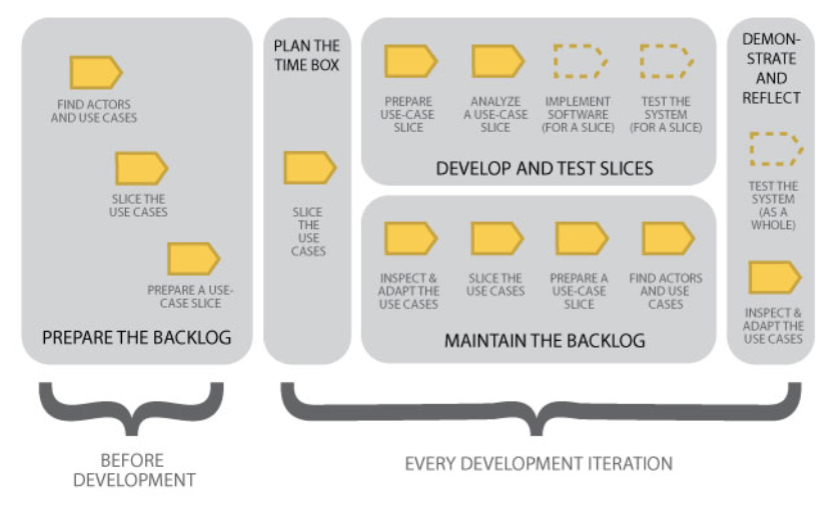
\includegraphics[width=0.7\textwidth]{figures/uc20_flow}
\caption{\Gls{use_case} 2.0 activities for iterative development approaches \cite{jacobson2011usecase}.}
\label{fig:usecase20:flow}
\end{figure}


\subsection{Use Cases, Use Case Flows and Use Case Slices}
\Glspl{use_case} are the core concept in Use Case 2.0. In addition to the original \gls{UML} specification, \glspl{use_case} are described as cards including the attributes Priority, Release, Size and Complexity. The MoSCoW scheme \cite{moscow} (Must, Should, Could, Won't) is used for priorisation. After the initial requirement analysis, \glspl{use_case_slice} are generated usually including flows, tests and an estimation of the development. In this step the different \glspl{Actor} are identified and test cases are specified. To do so, the \glspl{use_case_slice} are analysed regarding the interaction of system elements. They are then going to be implemented and tested with the previous defined test scenarios (\glspl{unit_test} and \glspl{integration_test}). Finally the whole system will be tested with \glspl{e2e_test}.

\Glspl{use_case} capture and identify the different goals of a system by telling a story on how to achieve a specific goal. This allows an easy communication of requirements of a system. \cite{jacobson2011usecase}

\textbf{\Glspl{use_case_flow}} define how the interaction between actors and the system proceeds. Usually there is a standard flow, and alternative (error / exception handling) flows. 

\textbf{\Glspl{use_case_slice}} are the final development tasks. They will be generated out of the use case flows and can be independently implemented as a single iteration step. They are based on flows and test cases. Further test cases are usually generated during the implementation to react on system specific scenarios and test requirements.


\subsection{Test Driven Development}
\label{sec:tdd}
\Gls{TDD} encourages simple designs and modularity of software products \cite{tdd}. Many companies therefore employ a \gls{TDD} process. This project uses \gls{RoR} which has test driven mechanics build in its core framework (\texttt{rspec}). In combination with the introduced Use Case 2.0 approach, \gls{TDD} can be easily used to ensure correctness between the specification of a \gls{use_case} and the actual implementation. In general \gls{TDD} is constructed out of following steps which are applied iterative: 

\begin{enumerate}
	\item Adding a test.
	\item Running all test and seeing the recently added test fail.
	\item Implementing the actual feature.
	\item Running the tests again and make them pass.
	\item Refactoring of the written code.
\end{enumerate}


One key component in \gls{TDD} is to keep it short and simple (KISS principle), which results in small, testable and reusable modules in a software and usually leads to better code quality. As the software will be developed in iterative steps, the progress is easily trackable and although changes are made to already existing features, the integrated tests for the previously implemented functionality ensures the continuous integrity of the overall system.  

In our case \glspl{unit_test}, \glspl{integration_test} and \glspl{e2e_test} have been used to test the overall system. As described in \autoref{sub:technical} a \gls{CI} system has been set up to ensure the integrity of the system. The implemented \glspl{e2e_test} are basically described by the standard- and alternative-flows that are attached to each \gls{use_case} as defined in \autoref{sub:use_cases}. The individual tests that were executed can be found in \autoref{sub:test_suit} in the appendix.


